\documentclass[a4paper,fleqn,twoside,12pt]{article}

%%%%%%%%%%%%%%%%%%%%

\usepackage[]{geometry}
\usepackage[latin1]{inputenc}
\usepackage[UKenglish]{babel}
\usepackage[UKenglish]{isodate}
\usepackage{amsmath}
\usepackage{amsfonts}
\usepackage{amssymb}
\usepackage{amsthm}
\usepackage{graphicx}
\usepackage{chngpage}
\usepackage{calc}
\PassOptionsToPackage{hyphens}{url}
\usepackage{hyperref}
\usepackage[nameinlink]{cleveref}
\usepackage{fancyhdr}
\usepackage{titletoc}
\usepackage[explicit]{titlesec}
\usepackage{natbib}
\usepackage[dvipsnames]{xcolor}
\usepackage[sc]{mathpazo}
\linespread{1.05} 
\usepackage[T1]{fontenc}
\usepackage{minted}

%%%%%%%%%%%%%%%%%%%%

\hypersetup{
	colorlinks=true,
	linkcolor=black,
	urlcolor=black,
	citecolor=black
}

\setlength{\parindent}{0mm}
\setlength{\parskip}{\medskipamount}
\renewcommand\baselinestretch{1.2}

\cleanlookdateon

\pagestyle{plain}
\renewcommand{\headrulewidth}{0.0pt}

\makeatletter
\fancypagestyle{plain}{
	\fancyhf{}
	\fancyhead[LE]{\thepage}
	\fancyhead[RE]{\textit{\@author}}
	\fancyhead[RO]{\thepage}
	\fancyhead[LO]{\textit{\@title}}
}
\makeatother

%%%%%%%%%%%%%%%%%%%%

\author{Your name}
\title{Project title}

\begin{document}

\makeatletter
\begin{titlepage}

\textbf{\Huge \@title} \\[1.5cm] 
\Large \textbf{\@author} \\
Department of Computer Science \\
University of Warwick \\

\vfill 

\begin{adjustwidth}{-\oddsidemargin-1in}{-\rightmargin}
    \centering
    
\includegraphics[width=\paperwidth]{line.png}
\end{adjustwidth}

\vspace*{-3.5cm}

\end{titlepage}
\makeatother

\pagestyle{plain}
\section{Introduction}\label{sec:introduction}

Bias is the overrepresentation of a particular topics in an individuals social media feed. This bias could be representative
of the individuals interests, or it could be representative of the interests of the social media platform. The latter is where
the notion of bias becomes complicated. Is my feed bias if it shows me only posts on topic A, if the only posts on the 
social media platform are of topic A? For the purpose of this report, we will take the stand that bias refers to the deviation from
the "norm".\\
\textbf{Bias Definition:} the deviation of a users social media feed from the distribution of available posts.

Bias in social media can easily be seen by comparing users' social media. In fact, I can show this with ease by just taking a look at my
Instagram's "Explore page", and compare it to another's.
\newpage
\begin{figure}[htbp]
    \centering
    
\includegraphics[height=80mm]{../images/ig4u.jpg}
    \caption{My Instagram for you page}
    \label{fig:ig4u}
\end{figure}

Here we can notice a few common themes/biases: 1. Food, 2. Formula 1, 3. Memes. We want to be able to identify these biases for users
so they can get an overview of the type of content they are receiving from social media.\\
With social media recommender systems programmed to entice users with content they will enjoy (\cite{recommenderSystems}), it is common for similar groups of posts
to be observed by a user if they have recently liked, commented, or viewed similar posts (\cite{instagram_how_nodate}).\\
Although the content in the feed only shows a small number of topics, we can not guarantee bias, as we are unaware of the 
distribution of all posts on the platform.

\newpage

\begin{figure}[htbp]
    \centering
    
\includegraphics[height=80mm]{../images/ig4u2.png}
    \caption{Another Instagram for you page}
    \label{fig:ig4u2}
\end{figure}

This for you page shows very different content to the previous one; there is a lot of sport/gym posts and absolutely no
posts on food. This helps to show that bias exists in social media.\\
\textbf{Proof}:
Let us assume that no bias exists in these examples.
Then simultaneously, the following must be true:
\begin{itemize}
    \item The posts in figure \ref{fig:ig4u} is representative of the entire distribution of posts on the social media site.
    \item The posts in figure \ref{fig:ig4u2} is representative of the entire distribution of posts on the social media site.
\end{itemize}

This, trivially, can not be true due to the fact that the two pages show differing content. $\qed$\\\\

This project attempts to show how bias is affected by how a user interacts with social media.
There are a couple of challenges to this project. The first being, even though we have a definition of bias,
we need a way to measure it. This involves creating a model to detect what topic a post is about and figuring
out how to identify the distribution of topics on a social media site. The second challenge is to setup rules that
represent different strategies users can use to interact with social media. We can then implement these rules
and analyse the change in topics over time.


\subsection{Related work}

\subsubsection{Pythia - \cite{Pythia}}
Pythia is an automated system for short text classification. It makes use of Wikipedia structure and articles to identify
topics of posts.
Essentially, "Wikipedia contains articles organized in various taxonomies, called categories". Pythia then goes on to use
this information as their training data as well as handling sparseness in posts on social media.

\subsubsection{Topic tracking of student-generated posts - \cite{TopicTracking}}
This paper proposes a solution for determining valuable information/topics discussed in student forums on online courses.
It uses a model called "Time Information-Emotion Behaviour Model" or otherwise called "TI-EBTM" to detect key topics discussions
, keeping in mind the progress of time throughout the forum.\\
Although this paper specializes in academic online forums, the approaches made could be relevant and useful for this project.

\subsubsection{Topic classification of blogs - \cite{husby2012topic}}
This paper uses Distant Supervision - 'an extension of the paradigm used by (\cite{snow}) for exploiting WordNet to extract hypernym (is-a) relations between entitities'
- to get training data via Wikipedia articles. Then trains their own designed model on this data to be able to classify topics via a
multi-class recognition model (69\% accuracy) and via a binary classification model (90\% accuracy).

\subsubsection{BERT - \cite{bertmodelling}}
This paper analyses BERT (as well as modified BERT models such as RoBERTa) and how they can be used for text classification.
The data used in this paper is a set of scientific papers that are classified into 7 different categories.\\

The paper shows that using a Feedforward Neural Network (FNN) on top of BERT can achieve a 91.76\% accuracy on the dataset.
This is a very high accuracy, and shows that BERT can be used for text classification.\\

\subsection{Objectives}

This project will require a topic detection model to be built and to perform some data analysis.
An extension for this project will be to create a Chrome Extension.

Below are the objectives for this project (Objectives in green are completed):

\begin{itemize}
    \item Build a topic detection model
    \begin{itemize}
        % make item green
        \item \textcolor{green}{Research possible models}
        \item \textcolor{green}{Gather data for model training}
        \item \textcolor{green}{Iterate over making and training models}
        \item Decide chosen model
        \item Train model on larger dataset
        \item Assess models accuracy and performance
        \item Include other information in the model (e.g. image/media attached in posts)
    \end{itemize}
    \item Data analysis
    \begin{itemize}
        \item Determine the distribution of topics on social media - aka the "norm"
        \item Create a set of rules to represent different strategies users can use to interact with social media
        \item Implement these rules and analyse the change in topics over time
        \item Compare the results of the rules to the "norm"
        \t\item This may require the use of a mathematical model to determine differences over time-series data
    \end{itemize}
    \item EXTENSION: Chrome Extension
    \begin{itemize}
        \item Design UI for extension
        \item Implement UI design
        \item Gather data from social media sites from the extensions frontend
        \item Create an API that receives post information and returns a set of most represented topics
        \item Connect extension to API
    \end{itemize}
\end{itemize}
\section{Background}
\label{sec:background}

Your literature review goes here. discusses the advantages of functional programming by exploring \emph{e.g.}\ lists, trees, and noughts and crosses in a functional programming language. 

\section{Progress}
\label{sec:progress}
\subsection{Weeks 1-2}
During the first 2 weeks of term time was spent on the Specificationa as well as attempting to establish a strong
base to the project in which I can build on for the rest of the project.

\begin{figure}[htbp]
    \centering
    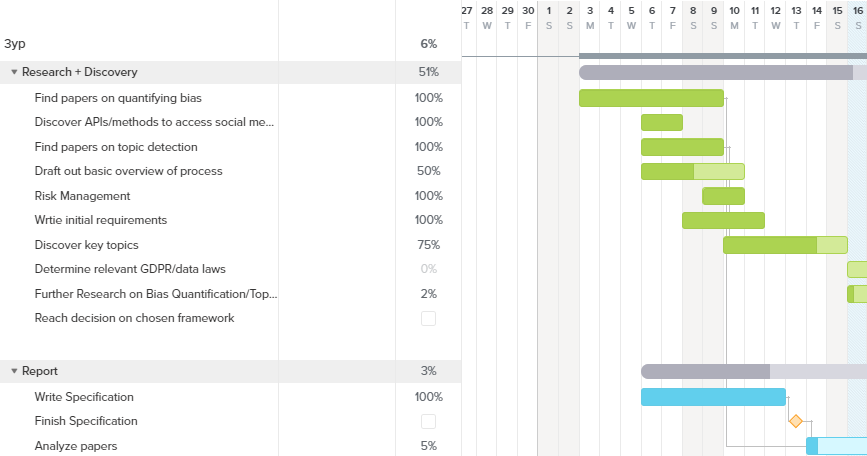
\includegraphics[width=0.5\textwidth]{../images/timetableweek1-2.png}
    \caption{Timetable for weeks 1-2}
    \label{fig:timetableweek1-2}
\end{figure}

As seen from this figure I met most of the deadlines set for the first 2 weeks of the project. I did miss some deadlines
Including: Drafting an overview of the process; Discovering key topics; and starting looking into GDPR and Data Protection laws.
Although it would have been beneficial to have achieved the latter 2 in the list above, the first objective was probably infeasible
for the first 2 weeks of the project - as further research is required to determine where I want this project taking.\\\\

I also completed a few extra tasks slightly early this week. I established an API connection to Twitter as well as reading up on
API access to Facebook and Instagram. As mentioned in my specification, I am going to stick with using Twitter as a base for
this project but may look into using Facebook and Instagram as well.\\\\

Finally I started looking more into the papers I laid out in the spec. Specifically looking into Pythia and how they overcome
the challenge of twitter posts usually being short and not containing much information.

\subsection{Weeks 3-4}
During weeks 3 and 4, time was spent time was spent further working on establishing the goals of the project. It was
decided that the project would be split into 2 parts. The first part would be to create a system that can be used to
analyse twitter posts and determine the topic of the post. I chose to go with a similar method used in Pythia \cite{Pythia}.
The latter stages of the project would involve using the system and analyse how different social media "strategies" affect
the topical bias of a users feed.\\\\

Below is the timetable for weeks 3-4.

\begin{figure}[htbp]
    \centering
    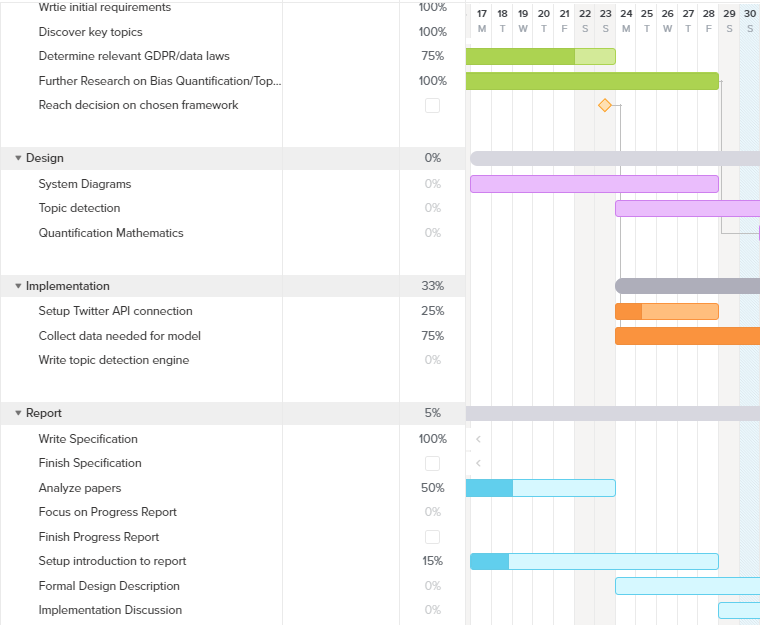
\includegraphics[width=0.5\textwidth]{../images/timetableweek3-4.png}
    \caption{Timetable for weeks 3-4}
    \label{fig:timetableweek3-4}
\end{figure}

As seen from the timetable above, I did not meet all of the deadlines set for weeks 3-4; due to needing to complete more
research on other methods of topic detection (such as Formal Concept Analysis, Clustering, and Latent Dirichlet Allocation),
I spent the week deciding which of these methods would be preferred (As mentioned above).

On top of this, I also gathered the Wikipedia data required for the training of the system. This involved:
\begin{itemize}
    \item Connecting to the Wikipedia API
    \item Searching for the decided upon categories
    \item Selecting 100 pages for each category
    \item Performing some preprocessing on the data
    \begin{enumerate}
        \item removing punctuation
        \item removing numbers
        \item removing excessive whitespace (leaving only spaces)
        \item removing Stopwords
    \end{enumerate}
\end{itemize}
def: Stopwords are words that are commonly used in the English language, but are uninformative \cite{sarica2021stopwords}.\\\\

This process gave us a total of $24,000$ sentences at around $1,000$ per category.


\subsection{Weeks 5-6}
During weeks 5 and 6, time was focussed around BERT. BERT, which stands for Bidirectional Encoder Representations from Transformers,
is a modern model which focusses on the task of language modelling. It is a pre-trained model which can be used to perform more precise
tasks after being fine-tuned \cite{devlin_bert_2019}. Fine-tuning of the model is done by adding a classification layer on top of the
model and training the model on a specific task.\\

The model was fine-tuned on the Wikipedia data gathered in the previous weeks. The model was trained on 24 categories, including:
Politics, Sports, Food, etc. The model was trained for 6 epochs, with a batch size of 32. The single output layer used the
softmax activation function. The model was trained using the Adam optimizer with the sparse categorical cross entropy loss function.\\

The data was split into 80\% training data and 20\% testing data. The model was trained on the training data and then tested on the
test data. Initially, the model was not very impressive, only achieving around 40\% accuracy.
% Insert figure, move onto next page if needed

\begin{figure}[htbp]
    \centering
    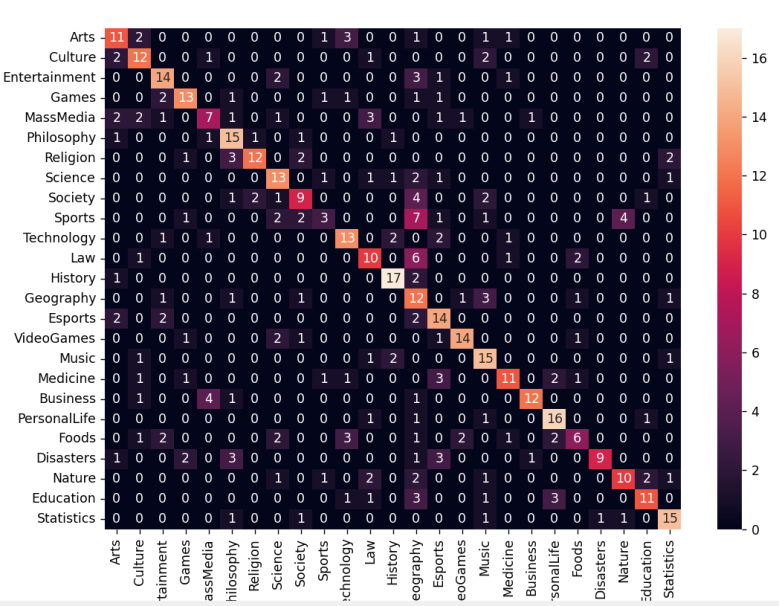
\includegraphics[width=0.5\textwidth]{../images/wiki-confusion.png}
    \caption{Confusion matrix on the Wikipedia data}
    \label{fig:wikiconf}
\end{figure}
Further analysis of the data showed that
the data was of a poor quality; even after the processing, the data still contained meaningless sentences. Take for example:
"51 (1): 209-220.", there is no way of identifying the topic of this sentence. On top of this, the data seemed to be too formal to
be used for analysing social media. Because of these facts, the decision was made to not use Wikipedia data for the training and instead
use Reddit data.\\
Reddit data was chosen as it is a more informal platform and is more likely to contain sentences that are formatted similarly to
other social media sites.\\
The same process as laid out in the previous weeks was followed. The data was gathered, preprocessed. The model was trained and tested
and with the reddit data, had a much higher testing accuracy of around 60\%.
\newpage
\begin{figure}[htbp]
    \centering
    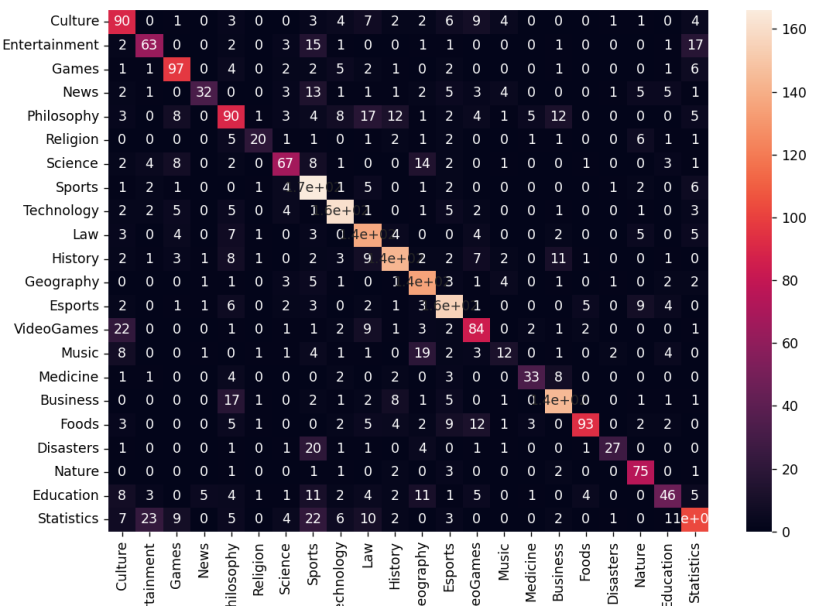
\includegraphics[width=0.5\textwidth]{../images/reddit-confusion.png}
    \caption{Confusion matrix on reddit data}
    \label{fig:reditconf}
\end{figure}

\subsection{Weeks 7-8}

\section{Project management}

Include a timetable (in 2 week chunks) for the remainder of the academic year, up until the submission deadline.

\bibliographystyle{./plainnat}
\bibliography{bibliography}

\end{document}